\documentclass{beamer}
\usefonttheme[onlymath]{serif}
\usepackage{amsmath}
\usepackage{amsfonts}
\usepackage[export]{adjustbox}
\usepackage[utf8]{inputenc}


%Information to be included in the title page:
\usecolortheme{seahorse}
\title{Reading Papers}
\author{Thomas Bayes}
\institute{
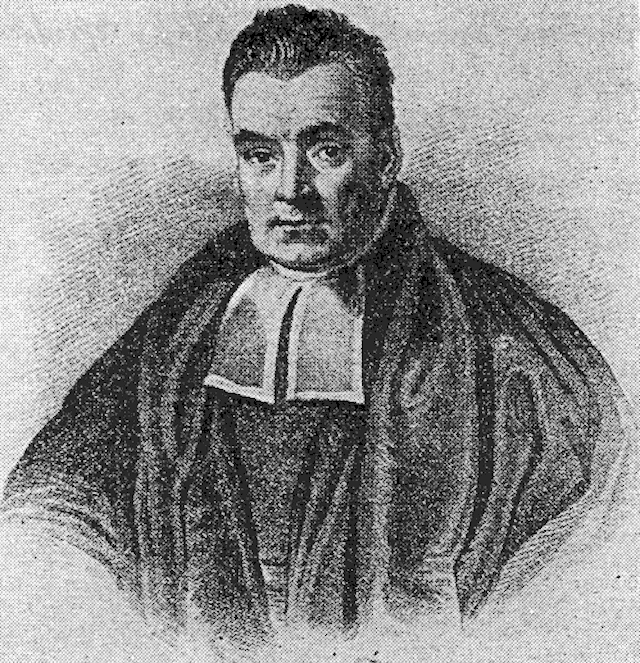
\includegraphics[height=.3\textheight]{../bayes.png}%
}
\date{\today}

    
\begin{document}
    
\frame{\titlepage}

\begin{frame}{Deep Probabilistic Programming\cite{tran2017deep}}
\begin{itemize}
\item You can take a DL model and make it probabilistic. (Section 3 assign prior probability on the parameter $\theta$ and infer the posterior.)
\item You can integrate the DL module in probabilistic models. (Section 4 introduced variational autoencoders.)
\item Advantages from probabilistic models(Section 5.1) 
\item Advantages from deep models(Section 5.2)
\end{itemize}
\end{frame}



\begin{frame}[allowframebreaks]{References}

\bibliographystyle{apalike}
\setbeamertemplate{bibliography item}[article]
\bibliography{ref}
\end{frame}
\end{document}